\vspace*{-0.5cm}
Le câblage du cryostat consiste en deux parties: 
\paragraph*{Les câbles DC: }ils véhiculent les signaux continus. Au nombre de 17, ils sont thermalisés à chaque étage pour limiter le bruit thermique.
\paragraph*{Les câbles coaxiaux: }les deux grilles rapides, le signal d'entrée et le signal de sortie. Ils font l'objet de beaucoup d'attention, afin d'avoir les meilleures mesures possibles.

\vspace*{0.2cm}
\begin{figure}[h]
    \begin{center}
        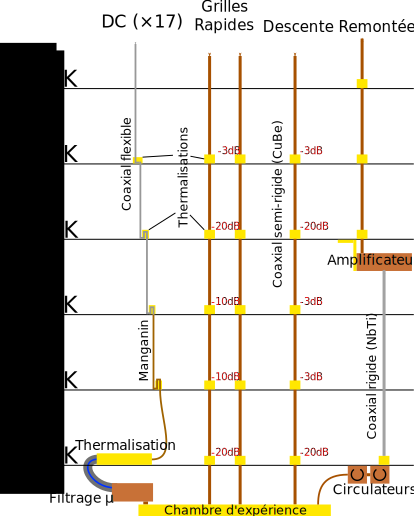
\includegraphics[width=0.7\textwidth]{Images/Cablage_schema}
        \caption{Schéma de câblage de l'expérience}
        \label{cablage_schema}
    \end{center}
\end{figure}




\section{Choix des matériaux}
Parlons tout d'abord des câbles de descente. Ceux-ci véhiculent le bruit thermique d'étage en étage, ce que nous voulons limiter au maximum.

Nous faisons donc le choix de câbles atténuant le signal afin de limiter l'apport de bruit. Ceci permet en plus de limiter les ponts thermiques entre étages dûs à la conductivité des câbles.
\newline

Les câbles DC sont alors:
\begin{itemize}
    \item des câbles coaxiaux souples entre 300K et 800mK, peu résistifs (le signal est suffisant pour avoir un bon rapport signal/bruit)
    \item des câbles de Manganin, très résistifs ($\sim45\Omega/m$), jusqu'à 20mK (l'étage le plus froid)
    \item des câbles peu résistifs ($\sim0.4\Omega/m$) jusqu'à la chambre d'expérience
    \newline
\end{itemize}

et les câbles RF coaxiaux semi-rigides de descente sont:
\begin{itemize}
    \item en Cuivre-Béryllium, thermalisé à chaque étage, jusqu'à 20mK. Le CuBe est beaucoup plus résistif que le Cuivre.
    \item en Cuivre jusqu'à la chambre d'expérience
\end{itemize}

Les câbles sont cintrés en "U" entre chaque étage, afin de limiter le passage des radiations au maximum. Ceci permet de plus d'avoir une certaine souplesse dans les câbles pour les connecter sans trop de difficultés.\newline

Enfin, on rajoute à chaque étage un atténuateur (valeur en rouge sur le schéma). Ceci permet d'envoyer en amont du cryostat un signal très fort, qui détruirait les échantillons, pour avoir dès le départ un rapport signal/bruit très bon.


\paragraph*{Pour le câble de remontée,}on raisonne différemment: il faut atténuer le signal le moins possible, jusqu'à l'amplificateur haute fréquence qui est situé à 4K (sa température nominale de fonctionnement). Un câble rigide de Niobium-Titane est alors utilisé.

Afin de limiter le "retour" de signal de l'amplificateur par ce câble, on thermalise deux circulateurs à 20mK. On utilise des câbles de Cuivre pour les connexions avec la chambre d'expérience.






\section{Thermalisation électronique}
Une grande partie du bruit provient de la température électronique. Si les câbles ne sont pas bien thermalisés, on risque de ne mesurer qu'un bruit à 300K.
\newline

Les câbles coaxiaux sont thermalisés à chaque étage du cryostat par des pinces, reliées par des câbles de cuivre jusqu'aux platines du cryostat. L'ensemble des pièces est bien sûr doré pour avoir les meilleurs contacts thermiques possibles ; les pores des parois en contact sont bouchées par de l'Apiezon N, à l'instar de la pâte thermique de nos processeurs.
\newline

Les câbles DC sont thermalisés à chaque étage par des presses dorées grâce à de la Stycast. Cette époxy permet une très bonne thermalisation des câbles fins aux presses dorées et montées sur les platines du cryostat.

Une thermalisation s'effectue aussi au niveau du boîtier de thermalisation où les câbles font des méandres afin d'assurer une bonne thermalisation électronique.

\begin{figure*}
    \centering
    \begin{subfigure}[t]{0.48\textwidth}
        \centering
        \includegraphics[height=1.2\textwidth]{Images/Thermalisation/DC}
        \caption{Fils de Manganin "stycastés" dans une presse dorée}
    \end{subfigure}%
    ~ 
    \begin{subfigure}[t]{0.48\textwidth}
        \centering
        \includegraphics[height=1.2\textwidth]{Images/Thermalisation/Coax}
        \caption{Câbles coaxiaux thermalisés}
    \end{subfigure}
    \caption{Thermalisation des câbles sur la platine du cryostat}
\end{figure*}

\newpage
\section{Filtrage des lignes DC}
En plus de la thermalisation, les lignes DC sont filtrées à l'étage 20mK. Un premier filtrage est effectué dans le boîtier de thermalisation à l'aide d'un filtre Passe-Bas RC du second ordre.

\begin{figure}[h]
    \begin{center}
        \includegraphics[height=0.4\textwidth]{Images/Thermalisation/DC3}
        \caption{Boîtier de thermalisation non soudé}
        \label{DC_Filtrage}
    \end{center}
\end{figure}

Un second filtrage est effectué grâce à l'Eccosorb. Cette résine composite à base d'époxy (même fabricant que la Stycast, mêmes solutions) absorbe très efficacement les micro-ondes résultant du bruit électronique.

Il a donc fallu mettre en place un petit boîtier, dans lequel nous faisons passer 17 câbles bleus de 80cm, compartimenté pour que l'Eccosorb n'abîme pas les prises lors du durcissement et des cycles de refroidissement.

J'ai donc décidé de dessiner des pièces en 3D sous OpenSCAD afin de former ces compartiments. Après quelques recherches, il est apparu que le matériau le plus utilisé en impression 3D, le PLA, peut être utilisé dans un cryostat (bien que jamais utilisé jusqu'ici).
\newline

En fait, beaucoup de matériaux ne sont pas compatibles avec de telles applications. Notamment, la faible pression dans le cryostat peut faire dégazer les matériaux (air dans les parois poreuses, ou des composants du matériau lui-même qui s'évapore). La plupart des matériaux élastiques sont dans ce cas.

De plus, certains matériaux peuvent ne pas supporter les cycles de refroidissement dans le cryostat. C'était le cas des précédentes séparations, qui ont alors cassé les câbles qui passaient au travers.

\subsection{Blindage des câbles DC}
En aval du boîtier de thermalisation, les câbles sont bien thermalisés et déjà bien filtrés. On ne voudrait donc pas laisser les câbles DC non blindés, au risque de recevoir des radiations, ne serait-ce que de l'étage à 100mK.

Une tresse métallique soudée à la masse entoure donc les câbles jusqu'au boîtier de filtrage micro-ondes. Celui-ci est directement branché sur la chambre d'expérience, les câbles restent donc isolés.

\begin{figure*}[t!]
    \centering
    \begin{subfigure}[t]{0.59\textwidth}
        \centering
        \includegraphics[height=0.633\textwidth]{Images/Thermalisation/Filtrage3D}
        \caption{Modélisation 3D des pièces dans le boîtier}
    \end{subfigure}%
    ~ 
    \begin{subfigure}[t]{0.39\textwidth}
        \centering
        \includegraphics[height=0.95\textwidth]{Images/Thermalisation/Filtrage}
        \caption{Boîtier de filtrage en place dans le cryostat}
    \end{subfigure}
    \caption{Boîtier de filtrage, rempli d'Eccosorb}
\end{figure*}





\section{Fabrication des câbles coaxiaux}
Comme je l'ai précisé plus haut, les signaux RF sont véhiculés par des câbles coaxiaux semi-rigides. J'ai donc procédé intégralement à la fabrication et la caractérisation de ces câbles.
\newline

La moindre imperfection des câbles coaxiaux se ressent fortement sur leur atténuation -- nous verrons cela plus tard -- , il faut donc les manier et les cintrer en faisant attention à ne pas les tordre.

\subsection{Étapes de fabrication}
Je vais ici décrire les différentes étapes de fabrication d'un câble coaxial connectorisé. Elles peuvent être trouvées en annexe dans le guide de câblage.

\paragraph*{Dénudage} Il faut dénuder quelques millimètres du câble pour souder la pin sur l’âme du
câble coaxial, à l'aide d'une petite scie.
\begin{figure}[h]
    \begin{center}
        \includegraphics[height=0.48\textwidth]{Images/Coax/1}
        \quad
        \includegraphics[height=0.48\textwidth]{Images/Coax/2}
        \caption{Dénudage d'un câble coaxial}
        \label{coax_denudage}
    \end{center}
\end{figure}

\paragraph*{Soudure de la pin centrale} On fixe une broche sur l’âme du câble, puis on serre le tout en
place. Pour prévoir la dilatation du diélectrique lors de la soudure, on place une petite entretoise juste avant la broche.
\begin{figure}[h]
    \begin{center}
        \includegraphics[width=0.60\textwidth]{Images/Coax/3}
        \caption{Pin centrale soudée sur le câble}
        \label{coax_soudure_centre}
    \end{center}
\end{figure}

\paragraph*{Soudure de la prise extérieure} On fixe sur la prise mâle une prise femelle factice qui permet de positionner à la distance correcte la prise mâle. Celle-ci a une partie mobile avec le pas de vis.
\begin{figure}[ht]
    \begin{center}
        \includegraphics[height=0.48\textwidth]{Images/Coax/4}
        \quad
        \includegraphics[height=0.48\textwidth]{Images/Coax/5}
        \caption{Soudure de la prise extérieure}
        \label{coax_soudure_exterieur}
    \end{center}
\end{figure}

\paragraph*{Fixation de l’isolant}  La dernière étape est de mettre un petit cylindre diélectrique entre la prise et la broche. On utilise alors une pièce creuse qui se visse dans le connecteur pour enfoncer le diélectrique.

\begin{figure}[ht]
    \begin{center}
        \includegraphics[width=0.60\textwidth]{Images/Coax/6}
        \caption{Fixation de l’isolant}
        \label{coax_fixation_isolant}
    \end{center}
\end{figure}

\paragraph*{Mesure du câble nécessaire} Après avoir connectorisé une extrémité du câble, il faut mesurer précisément la longueur de câble nécessaire. Il faut alors prendre en compte la longueur de câble qui se trouve dans le connecteur (sinon, il manquera quelques millimètres).

\begin{center}
    \includegraphics[width=0.40\textwidth]{Images/Coax/mesure}
    \label{coax_mesure}
\end{center}

\newpage
\paragraph*{Cintrage des câbles coaxiaux} Comme évoqué plus haut, les câbles doivent être cintrés entre chaque étage du cryostat. Néanmoins la fragilité des câbles nous impose de respecter un rayon de courbure minimal de 9mm.

Une cintreuse "sur mesure" permet de cintrer les câble correctement.

Pour les mesures, il faut prendre en compte 28mm de câble pour faire un demi-tour. Un cintrage en "U" nécessite alors 35mm de câble de plus qu'un câble droit.

\begin{figure}[h]
    \begin{center}
        \includegraphics[width=0.60\textwidth]{Images/Coax/cintrage}
        \caption{Câbles coaxiaux cintrés en "U" et connectés}
        \label{coax_cintrage}
    \end{center}
\end{figure}




\chapter{Caractérisation des câbles coaxiaux}

Maintenant que les câbles ont été cintrés et connectorisés, il faut mesurer leur caractéristique atténuation/fréquence. D'une part pour vérifier si les câbles sont utilisables, et d'autre part pour avoir les valeurs exactes d'atténuation afin de calibrer nos mesures à fréquence fixée.

L'appareil dédié à cette tâche est le VNA (Vector Network Analyzer) ou PNA (Performance Network Analyzer). L'équipe a récemment fait l'acquisition d'un PNA N5242 de Agilent.

Les graphes obtenus représentent l'atténuation en dB, qui est l'unité de mesure habituelle pour les câbles coaxiaux.
%TODO Finir le paragraphe
\begin{figure}[h]
    \begin{center}
        \includegraphics[width=0.65\textwidth]{Images/VNA}
        \caption{Le PNA de l'équipe}
        \label{PNA}
    \end{center}
\end{figure}

En se plaçant sur un canal de mesure, on effectue une calibration électronique (à l'aide d'un boîtier externe connecté au PNA) avec les câbles flexibles supplémentaires, puis on connecte notre câble coaxial.

\newpage
\section{Paramètres du PNA}
\begin{description}
    \item[Gamme de mesure :] 1GHz - 20GHz et 4-8GHz
    \item[Nombre de points :] 12801
    \item[Puissance :] -20dB et Power On
    \item[IF Bandwidth :] 1kHz
\end{description}

On effectue deux séries de mesure, entre 1 et 20GHz et entre 4 et 8GHz.

\section{Résultats attendus}

\begin{itemize}
    \item L'atténuation augmente avec la fréquence
    \item Elle est comprise entre -0.5dB et -2.5dB
    \item Jusqu'à 8GHz, l'atténuation doit être assez stable (peu de sinusoïdale) : L'essentiel des mesures est effectée entre 4 et 8GHz, d'où la série de mesures restreinte à cette gamme.
\end{itemize}

\begin{figure}[ht]
    \begin{center}
        \includegraphics[width=0.65\textwidth]{Images/Caracs/abime2.png}
        \caption{La caractéristique d'un câble correct(vert) et un abîmé (violet)}
        \label{Carac1}
    \end{center}
\end{figure}

Néanmoins un câble très cintré n'est pas forcément synonyme de mauvaise caractéristique.


\begin{figure*}[ht]
    \centering
    \begin{subfigure}[t]{0.40\textwidth}
        \centering
        \includegraphics[height=1.2\textwidth]{Images/Coax/Tres_cintre}
        \caption{Câble cintré à plus de 270\textdegree }
    \end{subfigure}%
    \begin{subfigure}[t]{0.6\textwidth}
        \centering
        \includegraphics[width=1.0\textwidth]{Images/Caracs/Tres_cintre}
        \caption{Caractéristique très bonne}
    \end{subfigure}
    \caption{Câble très cintré à bonne caractéristique}
\end{figure*}


\newpage
\section{Guide de câblage}
En complément du travail de câblage que j'ai effectué, j'ai écrit un guide de câblage détaillant les étapes à suivre afin de connectoriser un câble coaxial, ainsi que pour le caractériser.\newline

Celui-ci se trouve en annexe. Il détaille aussi la mise en place des boîtier de filtrage et l'utilisation du VNA.





